\section{System Architecture}
\label{sec:arch}

\subsection{Overview}
The system operates on a reactive sense-deliberate-act cycle, where each server-side sensing event drives a new iteration of the BDI loop.
Figure~\ref{fig:agent_architecture} sketches the high-level data flow.

\begin{figure}[H]
    \centering
    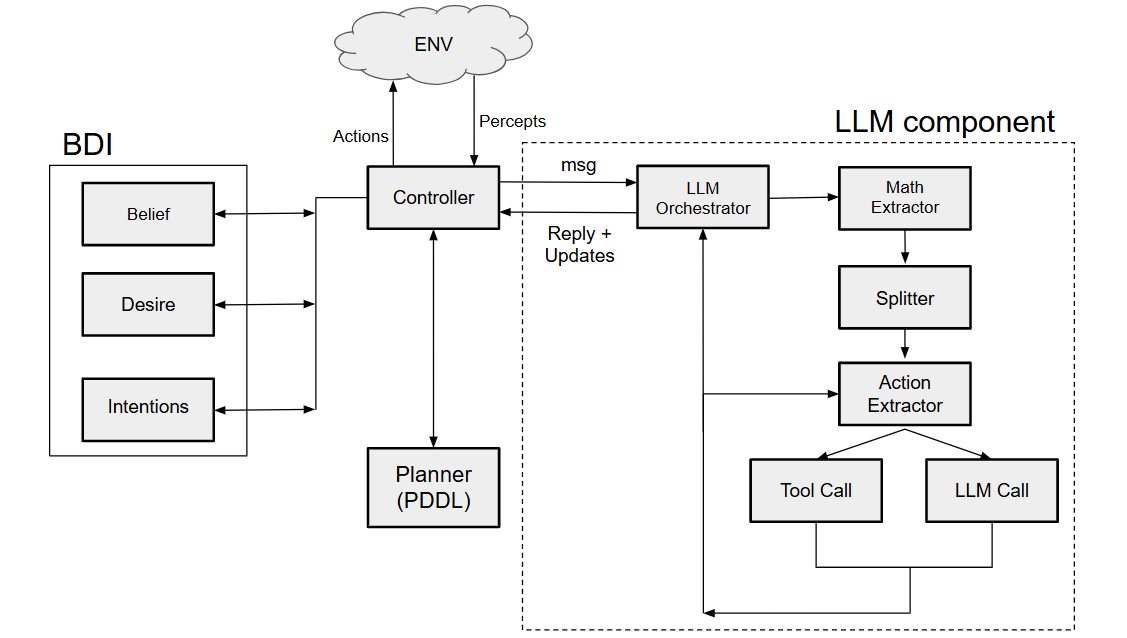
\includegraphics[width=1\textwidth]{images/agent_architecture.png} 
    \caption{Agent Architecture} 
    \label{fig:agent_architecture}
\end{figure}

The system comprises three main subsystems:
\begin{itemize}
    \item \textbf{BDI}: maintains world beliefs, generates desires, and commits to intentions.
    \item \textbf{Planning Component (PDDL)}: computes movement paths.
    \item \textbf{LLM Component}: interprets natural-language instructions and leverages a dedicated suite of \textbf{deterministic tools} (e.g., for mathematical evaluations) to inject updates into the BDI loop.
\end{itemize}

The entry point \texttt{main.ts} wires all components together, handles the WebSocket events, and runs the main BDI step function.

\subsection{BDI Agent Model}
The BDI layer is split across three files.

\paragraph{Beliefs (\texttt{BDI/Belief.ts}).} 
The belief layer implements the agent's belief update step, maintaining an internal representation of the environment under partial observability.
During initialization, the main socket handlers configure the agent parameters, build the static map, and initialize the agent's own position. After this setup, each sensing event updates the dynamic part of the world state, including parcels, crates, and other agents.

Beliefs are stored inside the \texttt{World} object as coordinate-indexed maps. When new observations arrive, \textbf{beliefs} are \textbf{updated}. Entities that are temporarily outside the observation range are not removed immediately; instead, they are kept for a short time using timestamp-based lifespans. This provides the agent with limited short-term memory, making its behavior more robust to partial observability.

The belief update also enriches the raw observations with task-relevant information. For example, opponent positions can be tracked over time to infer movement direction or stationary behavior, while crates positions are refreshed when visible and later used for obstacle modeling. In parallel, the main loop keeps an auxiliary state such as the list of carried parcels by the agent.

\textbf{Belief revision} allows the agent to avoid temporarily blocked cells even when no obstacle is explicitly observed. This accounts for dynamic obstructions, such as agents moving into a cell between sensing cycles (which are then corrected at the next \texttt{onSensing} event), as well as cells flagged as blocked via LLM-interpreted textual instructions.

Overall, the belief state is therefore not limited to the latest sensor reading. It combines persistent map information, short-lived memories of dynamic entities, and auxiliary runtime state needed by the BDI loop to select and execute intentions.

\paragraph{Desires (\texttt{BDI/Desire.ts}).} 
A Desire is represented as a tuple $\langle \text{type}, x, y, u \rangle$, where $u \in \mathbb{R}$ denotes its utility score. The agent generates three internal desire types:

\begin{itemize}
    \item \textbf{\texttt{go\_pickup}}: generated for each visible parcel that is not currently being carried. Its utility \ref{sec:pickup_utility} depends on the parcel reward, the distance required to reach it, and the distance from the parcel to the nearest delivery zone. The score is also reduced when opponents are close to the pickup location, using a competitive penalty based on the number of nearby agents.
    
    \item \textbf{\texttt{go\_delivery}}: generated when the agent is carrying at least one parcel. Its utility \ref{sec:delivery_utility} estimates the remaining reward obtainable by reaching the closest free delivery tile, subtracting the expected decay cost of the trip. Delivery tiles occupied by stationary opponents are penalized.
    
    \item \textbf{\texttt{explore}}: generated as a fallback behavior to guide the agent toward high-density spawn regions that have not been visited recently. Its score combines recency, BFS distance, spawn-cluster density, and opponent pressure \ref{sec:explore_utility}. Multiple exploration candidates are generated so that the agent can switch to an alternative target if one path becomes unreachable.
\end{itemize}

A fourth desire type, \texttt{go\_to}, is injected exclusively by the LLM component, as described in Section~\ref{sec:llm}. New atomic LLM tasks have to be inserted at this level of the architecture.

\paragraph{Intentions (\texttt{BDI/Intentions.ts}).} 
The \texttt{reviseIntention} function implements the agent's \textbf{intention revision} policy, which is executed at every BDI step. Based on the updated beliefs and a list of desires sorted by utility, this function determines whether the agent should maintain its current commitment or switch to a better candidate.

The control flow handles two main scenarios. If no intention is currently active, the agent automatically commits to the highest-utility desire. Conversely, if an intention is already active, its ongoing \textit{validity} is verified against the current world state. Specifically, delivery intentions remain valid only while the agent is carrying at least one parcel, whereas pickup intentions are kept only as long as the target parcel is still available on the map. Exploration intentions, on the other hand, are always considered valid and act as a fallback behavior when no other tasks can be performed. If the active intention fails its respective validity check, it is immediately discarded and replaced by the best available desire. Intentions can be \textbf{blocked} after a fixed number of failures and the agent automatically switch intention to the next best one. 

\TODO{Add here the LLM level 2 updates.}

\subsection{Planning Component}
The planning component enables the agent to compute a path toward a target tile. To evaluate the performance and efficiency of the planning subsystem, we implement a Breadth-First Search (BFS) algorithm as a baseline for shortest-path calculation and compare it against a classical automated planning approach using PDDL. 

\TODO{Update this section if PDDL is extended to handle crates or other dynamic domain objects.}

The PDDL-based module leverages the \textit{Fast Downward} planner, configuring it to use the $A^*$ search algorithm to determine the optimal path. Within this formalization, the planning domain defines the available actions as the movement capabilities of the agent, while the state space represents the grid tiles of the environment. 


\subsection{LLM Component}
\label{sec:llm}

The LLM component processes textual user inputs and extracts the structured information required to update the BDI agent's state. For this purpose, we selected the \textit{Llama-3.3-70B} model due to its advanced reasoning capabilities. To optimize performance and context window efficiency, we condition the model's short-term memory using concise system prompts paired with tailored \textit{few-shot examples} for each specific task.

The LLM component is designed to handle and execute a variety of tasks, which can be categorized into three levels of complexity:
\begin{itemize}
    \item \textbf{Atomic Special Missions:} Relatively simple and self-contained tasks. They do not require persistent state tracking solved by simple answering or modification to the intentions in the BDI component
    \item \textbf{Intermediate Special Missions:} Non-atomic, persistent tasks that remain active throughout the entire match. They require the implementation of dedicated data structure to force the agent to dynamically adapt its game strategy.
    \item \textbf{Coordination or Communication Missions:} High-complexity tasks that demand explicit communication channels among the two agents.
\end{itemize}

The core logic is managed by an orchestrator through the \textit{processMessage} function, which executes the following pipeline:
\begin{enumerate}
    \item \textbf{Mathematical Pre-processing:} The message is first passed to the \textit{mathExtractor} (first LLM call). It identifies nested arithmetic operations, replaces them with unique placeholders (e.g., $X1, X2$), and returns a structured JSON object. The orchestrator then invokes a deterministic \textit{calculate} tool to resolve these expressions and injects the actual results back into the text. This prevents LLM hallucinations and gracefully handles complex, nested calculations.
    \item \textbf{Utterance Splitting:} The cleaned message is processed by the \textit{splitter} component (second LLM call), which divides concatenated or complex queries into a list of independent sub-goals (e.g., splitting "go to tile 0,0 and tell me the square root of four" into two separate tasks).
    \item \textbf{Action Extraction and Execution:} Each sub-goal in the queue is evaluated by an \textit{action extractor} (third LLM call) to classify the intent and map it to a specific system tool. 
\end{enumerate}

Finally, based on the predicted action, the corresponding tool is executed. The orchestrator aggregates the results, returning both a textual answer (to be replied via chat) and a structured list of updates to be injected into the BDI component.

While this multi-step pipeline introduces a minor computational overhead due to consecutive LLM calls, it remains fully sustainable within the project's scope. The challenge constraints are relatively relaxed, as requests occur sporadically and do not require real-time, millisecond-range execution; this makes architectural robustness and accuracy preferable over raw speed. Moreover, this modular design allows for individual performance evaluation of each component, enabling targeted adjustments at every step.

The \textbf{tools} implemented to support the agent's actions are contained in a dedicated module that exposes the following functions:

\begin{itemize}
    \item \textbf{calculate}: A secure mathematical expression evaluator. Instead of using a dangerous global \textit{eval}, it parses the input string, validates it against a strict whitelist of allowed characters and syntax to prevent code injection, and executes the calculus using a safe subset of the native JavaScript \textit{Math} object (supporting functions like \textit{sqrt, pow, sin} and constants like $\pi$ and $e$).
    \item \textbf{getCurrentTime}: Retrieves the local date and time for a given city. It dynamically imports the external library \textit{city-timezones} to look up the correct timezone. The time formatting is handled natively via the JavaScript \textit{Intl.DateTimeFormat} API.
    \item \textbf{getMyPosition}: A utility function that reads the agent's current state and returns a formatted string with its coordinates $(x, y)$.
    \item \TODO{Add new tools if necessary}
\end{itemize}

All calculated answers and structured game-state updates are subsequently forwarded also to the \textit{only BDI} agent, ensuring it possesses all the necessary data to execute the required actions and successfully claim the points for the completed request.




